\chapter{Convertidor de Rampa Doble}

\begin{figure}[H]
    \centering
    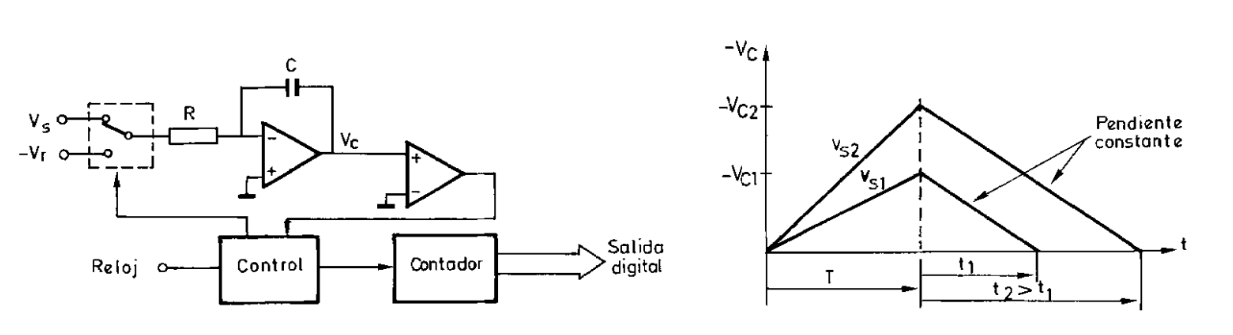
\includegraphics[width=0.75\linewidth]{Imagenes/Convertidor Doble Rampa.png}
    \caption{Convertidor A/D de doble rampa.}
\end{figure}

En los convertidores de doble rampa, se integra la señal de entrada $v_s$, constante, en un condensador durante un tiempo prefijado $T$, y luego se descarga el condensador hasta cero, empleando una corriente conocida determinada por la tensión de referencia, $V_r$. En la fase de integración, la tensión en el condensador alcanza un valor

\begin{equation}
    V_C = \frac{1}{\tau} \int_{0}^{T} - v_s dt = \frac{v_s}{\tau}T
\end{equation}

donde $\tau = R C$ es la constante de tiempo del integrador. La descarga hasta $0 V$, empleando la tensión de referencia $-V_r$, para establecer la corriente de descarga, dura un tiempo $t$ tal que

\begin{equation}
    0 - v_s = \frac{1}{\tau} \int_{T}^{T + t} -(-V_r)dt = \frac{V_r}{\tau} t
\end{equation}

De estas ecuaciones se obtiene

\begin{equation}
    t = T \frac{v_s}{V_r}
\end{equation}

Resulta, pues, que le tiempo que dura la descarga es proporcional a la amplitud de la entrada. Dado que el reloj con que se miden los tiempos y el condensador de integración son los mismos en la fase de carga y en la de descarga, su exactitud no influye en la precisión de la conversión, siempre y cuando permanezcan estables durante el tiempo de la conversión. La exactitud del convertidor depende sólo de la tensión de referencia y de los errores de cero internos. Este método de conversión es inherentemente lineal.
